
\documentclass[twoside,twocolumn]{article}

\usepackage{blindtext} % Package to generate dummy text throughout this template 

\usepackage[sc]{mathpazo} % Use the Palatino font
\usepackage[T1]{fontenc} % Use 8-bit encoding that has 256 glyphs
\linespread{1.05} % Line spacing - Palatino needs more space between lines
\usepackage{microtype} % Slightly tweak font spacing for aesthetics

\usepackage[english]{babel} % Language hyphenation and typographical rules

\usepackage[margin=0.5in,top=15mm,columnsep=10pt]{geometry} % Document margins
\usepackage[hang, small,labelfont=bf,up,textfont=it,up]{caption} % Custom captions under/above floats in tables or figures
\usepackage{booktabs} % Horizontal rules in tables

\usepackage{lettrine} % The lettrine is the first enlarged letter at the beginning of the text

\usepackage{enumitem} % Customized lists
\setlist[itemize]{noitemsep} % Make itemize lists more compact

\usepackage{abstract} % Allows abstract customization
\renewcommand{\abstractnamefont}{\normalfont\bfseries} % Set the "Abstract" text to bold
\renewcommand{\abstracttextfont}{\normalfont\small\itshape} % Set the abstract itself to small italic text

\usepackage{titlesec} % Allows customization of titles
\renewcommand\thesection{\Roman{section}} % Roman numerals for the sections
\renewcommand\thesubsection{\roman{subsection}} % roman numerals for subsections
\titleformat{\section}[block]{\large\scshape\centering}{\thesection.}{1em}{} % Change the look of the section titles
\titleformat{\subsection}[block]{\large}{\thesubsection.}{1em}{} % Change the look of the section titles

\usepackage{fancyhdr} % Headers and footers
\pagestyle{fancy} % All pages have headers and footers
\fancyhead{} % Blank out the default header
\fancyfoot{} % Blank out the default footer
\fancyhead[C]{MSc ACSE -5 Group Assessment 2022 $\bullet$ Jan 2022 } % Custom header text
\fancyfoot[RO,LE]{\thepage} % Custom footer text

\usepackage{titling} % Customizing the title section

\usepackage{hyperref} % For hyperlinks in the PDF

\usepackage{graphicx} %package to manage images
\usepackage{subfigure}
\usepackage{caption}
\usepackage{subcaption}
\usepackage{booktabs}
\usepackage{float}

\usepackage[table,xcdraw]{xcolor}
\graphicspath{ {./images/} }
%----------------------------------------------------------------------------------------
%	TITLE SECTION
%----------------------------------------------------------------------------------------

\setlength{\droptitle}{-4\baselineskip} % Move the title up

\pretitle{\begin{center}\Huge\bfseries} % Article title formatting
\posttitle{\end{center}} % Article title closing formatting
\title{LINEAR SOLVERS FOR DENSE AND SPARSE MATRICES} % Article title
\author{%
\textsc{yuna nakamura},
\textsc{ellya kanimova},
\textsc{niranjana sundararajan}
}
\date{\today} % Leave empty to omit a date
\renewcommand{\maketitlehookd}{%
% \begin{abstract}
% \noindent \blindtext % Dummy abstract text - replace \blindtext with your abstract text
% \end{abstract}
}

%----------------------------------------------------------------------------------------

\begin{document}

% Print the title
\maketitle

%----------------------------------------------------------------------------------------
%	ARTICLE CONTENTS
%----------------------------------------------------------------------------------------

\section{Introduction}

\lettrine[nindent=1em,lines=2]{L}inear Systems of the type \(A*X = B\)  that arise from the discretisation of a number of partial differential equations are a very common type of problem that requires robustly designed solvers that account for optimisations in both time and memory management. This matrix library can be used for such  implementations. Depending upon specific requirements and the nature of the linear system, different solvers each with their own set of properties are available to the user.\\
The solvers implemented in the project include both direct and iterative solvers. The direct solvers implemented include Gauss elimination with partial pivoting, LU decomposition and the Cholesky Method. The iterative methods include the Jacobi Method, the Gauss-Siedel Method and the Conjugate Gradient method.\\
Of the methods listed above, all are implemented for the dense matrix input and the conjugate gradient and Jacobi methods are implemented for the sparse matrix

%------------------------------------------------
\section{Code Structure and Design Decisions}
The figure below shows all the base classes in our library(in light blue) and the inherited classes (darker blue) with the dotted line indicating inheritance.\\
\begin{figure}[h]
\centering
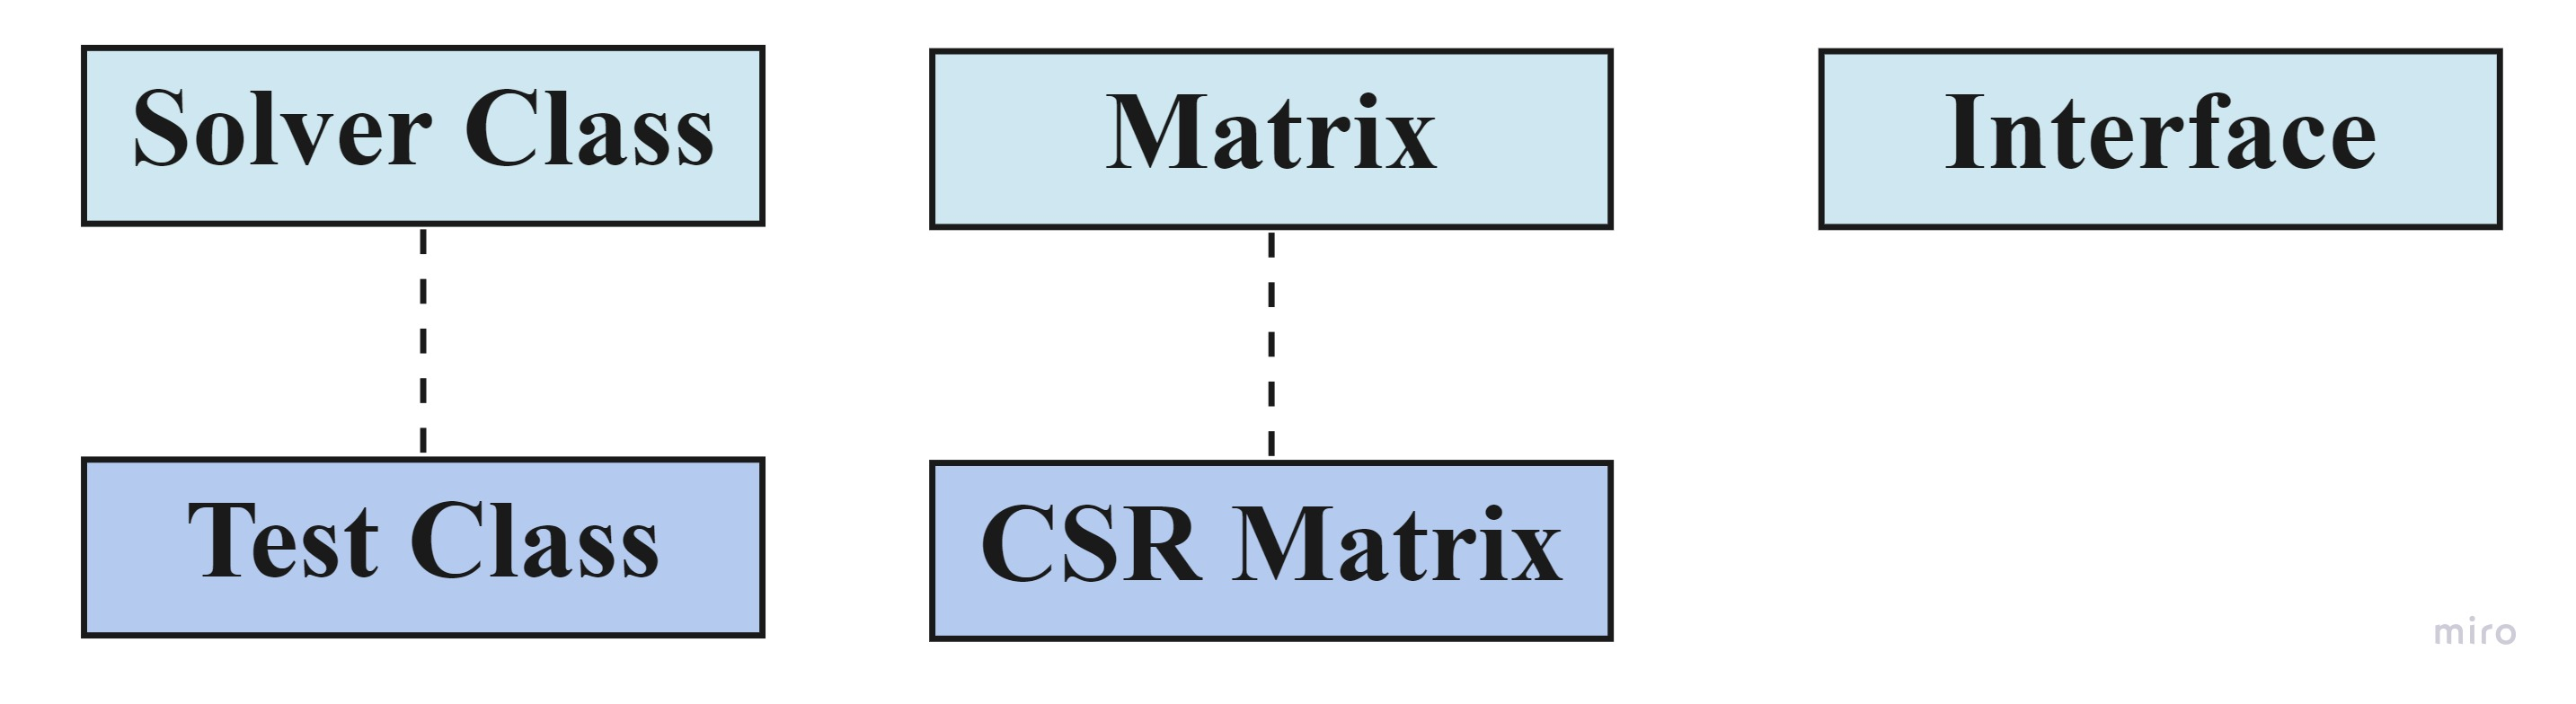
\includegraphics[height=2cm\textwidth]{images/Main Classes and Hierarchies.jpg}
\caption{All Classes and Hierarchies}
\end{figure}

In the current versions of the Matrix and CSR Matrix class, the implemented library has build upon the existing code with added functionalities. \\
While our code builds on the Matrix and CSR Matrix classes, the library implements three new classes - the Solver, the Interface and the Test classes with extensive functionalities needed to solve our linear systems. These functionalities are briefly illustrated in the charts on the right:

\begin{figure}[H]
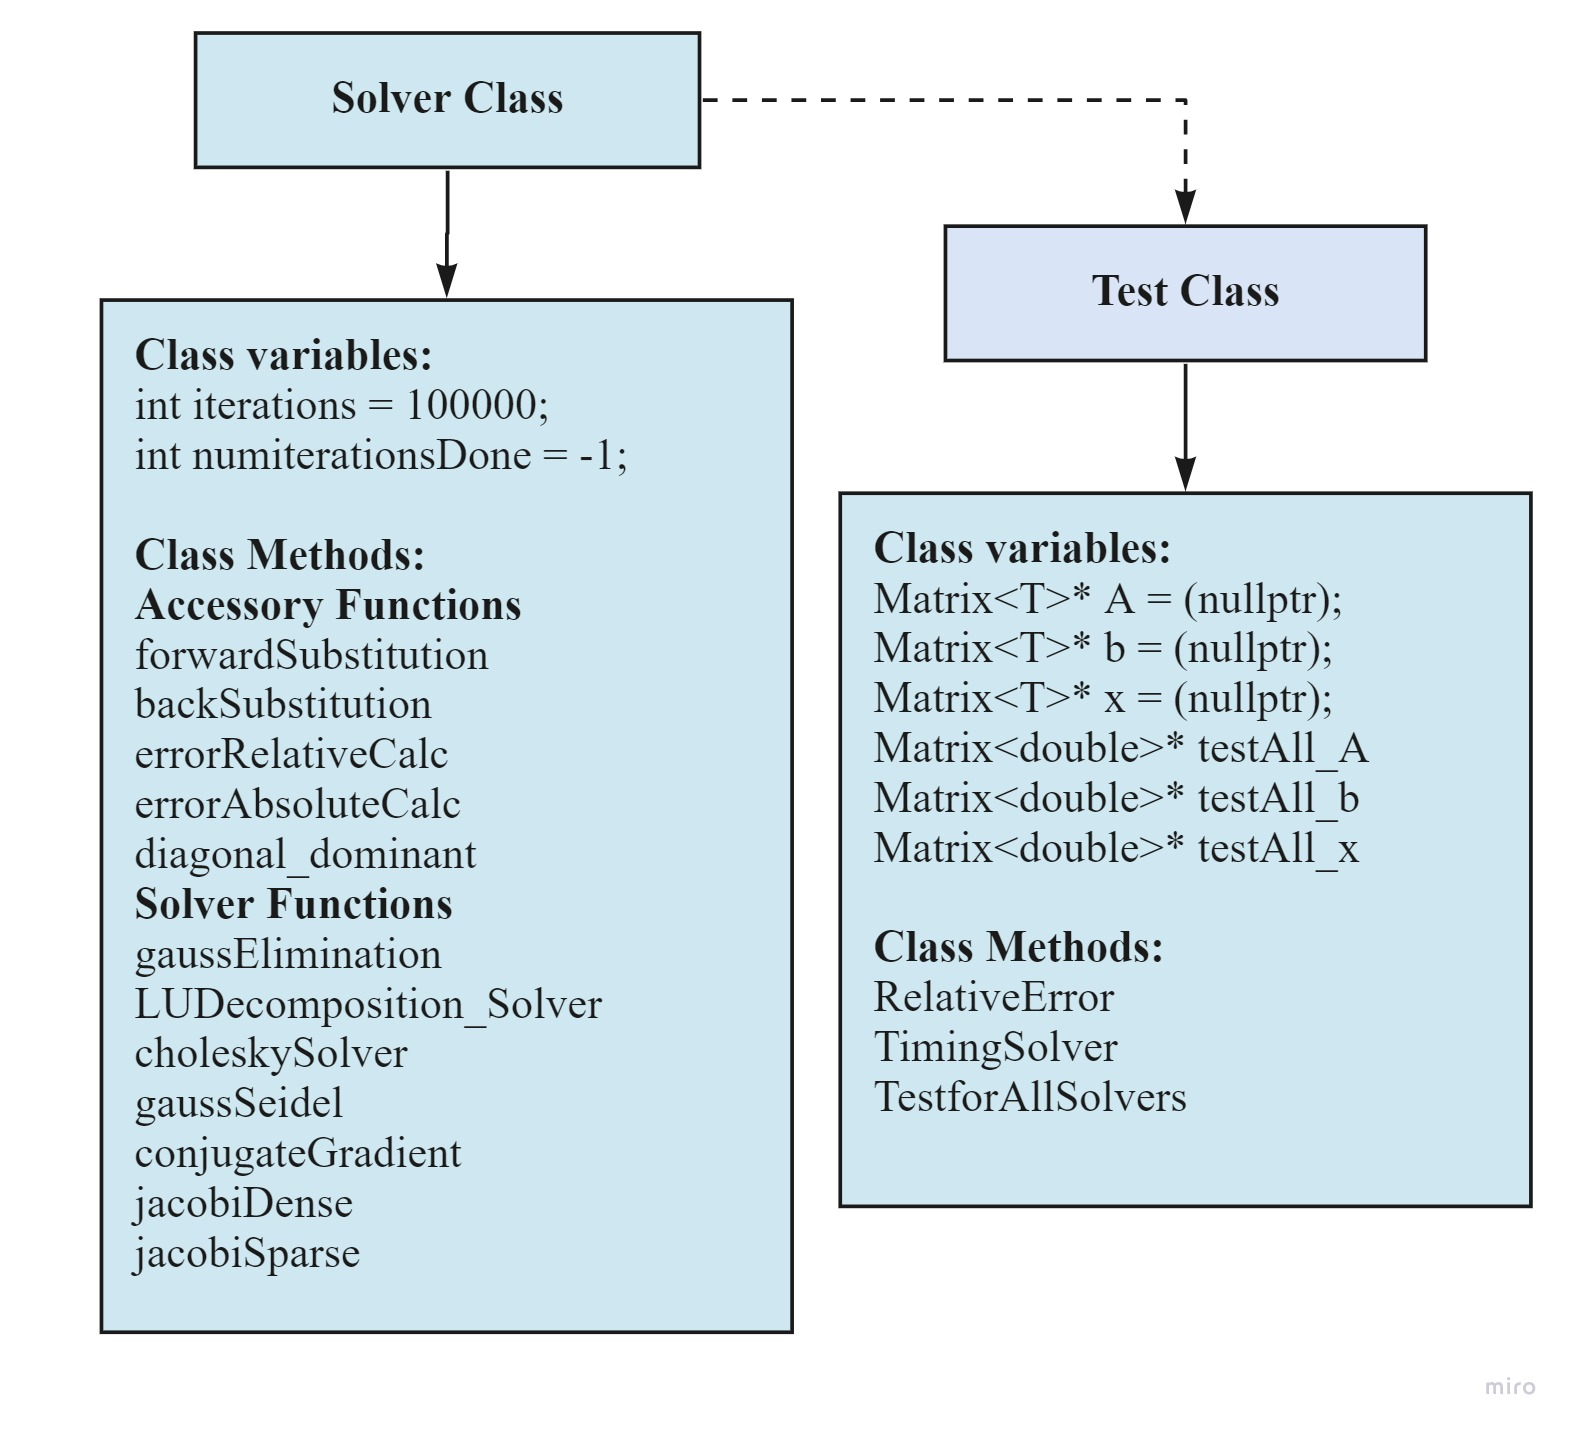
\includegraphics[width=0.5\textwidth]{images/solverandTest.jpg}
\caption{Classes Implemented to Extend Backend Functionalities}
\end{figure}

Further, an interface class is implemented as a frontend at the terminal to provide additional ease of testing and validation.
\begin{figure}[H]
\centering
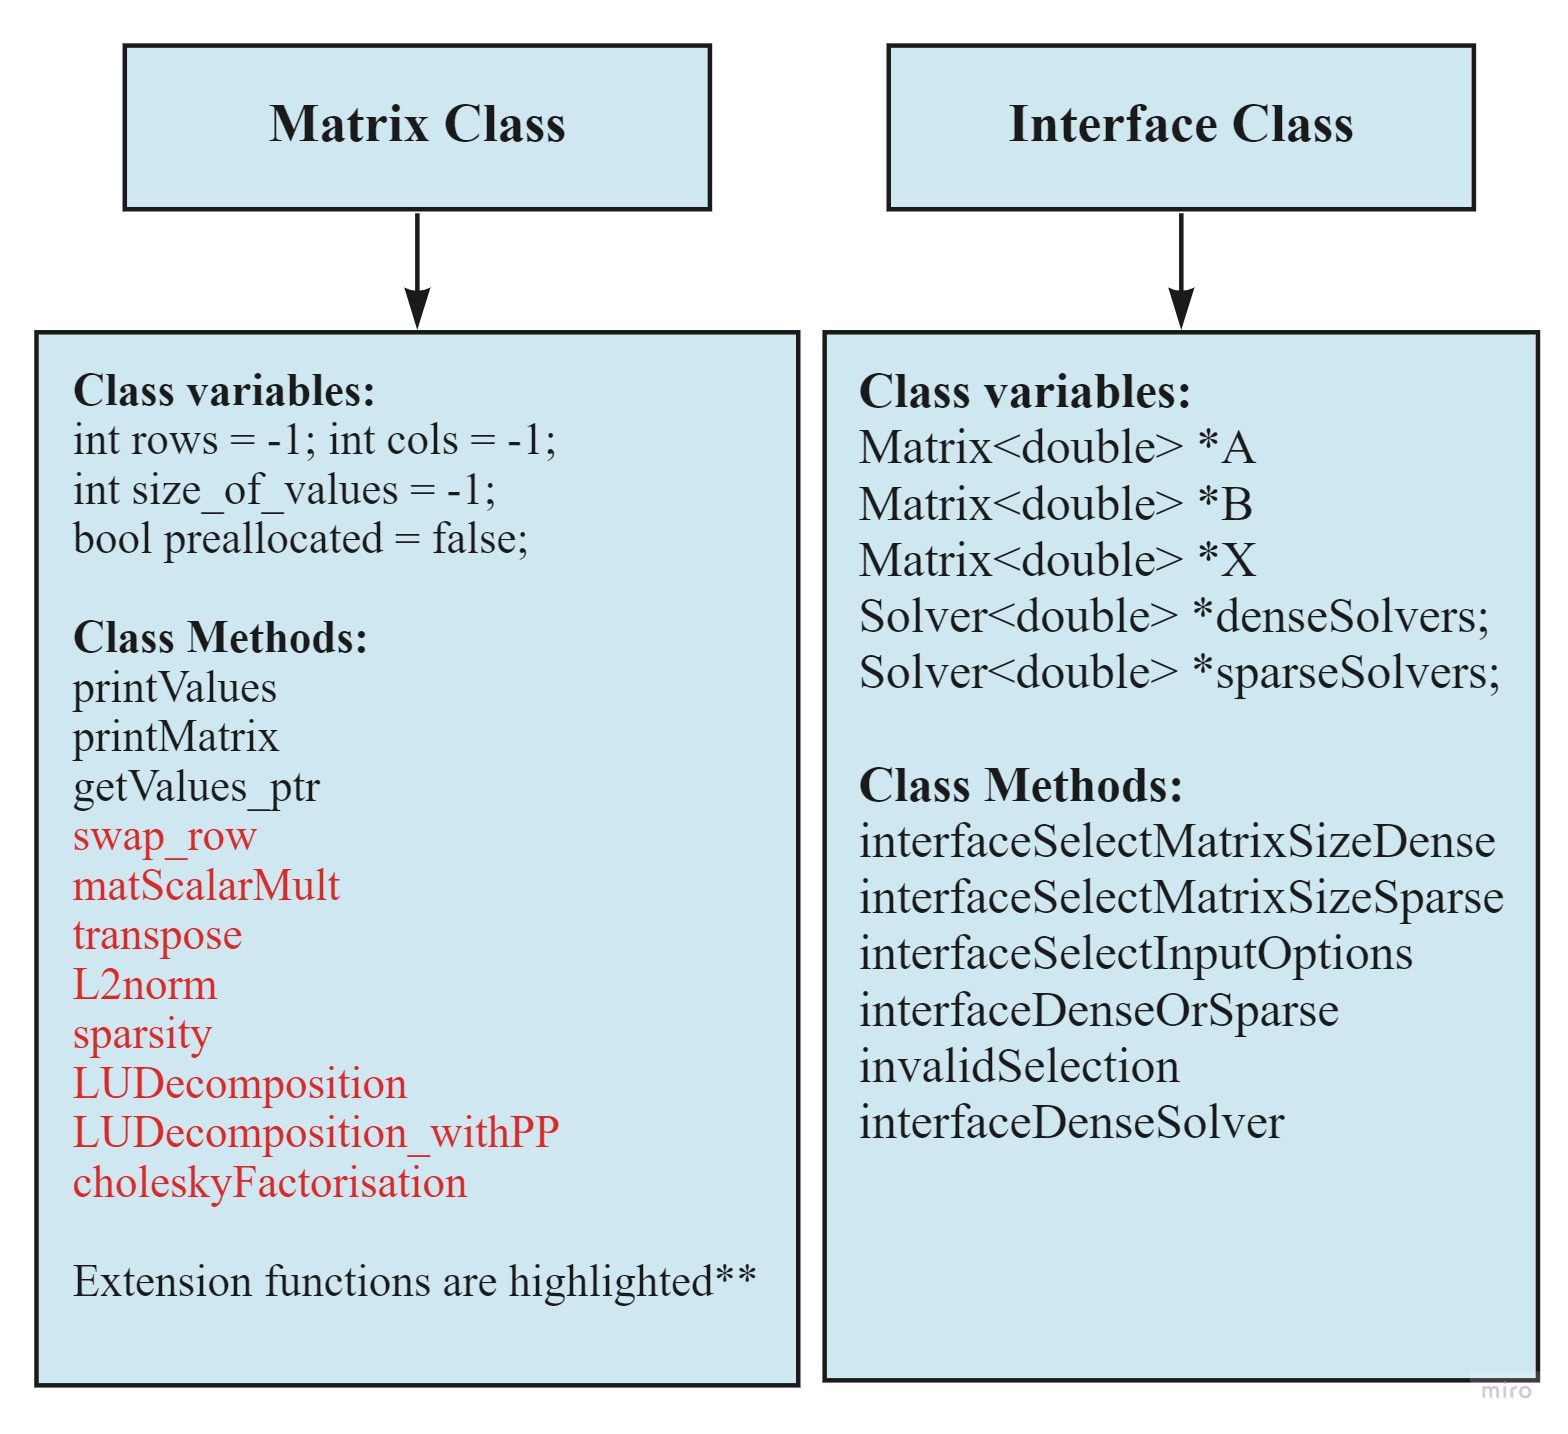
\includegraphics[width=0.45\textwidth]{images/Interface.jpg}
\caption{Extended Functionalities of Matrix Class and Classes Implemented to Add Frontend Tests}
\end{figure}
The library is implemented using various Object Oriented Programming design principles for efficient and sustainable code structure and maintainability. The following are few principles and their implementations in our library :
\begin{itemize}
    \item \textbf{Inheritance}: The Test class inherits from the solver class. This was a design decision to further simplify the usage of solver functions for both validation and performance testing of the solvers implemented. 
    \item \textbf{Templates}: All classes, except the interface class are templatised to allow for matrix inputs to be of preferred data types. This allows for both better memory management, flexibility for the user and performance.
    \item \textbf{Smart Pointers}: Smart pointers are used in the Matrix functions and classes within the library to ensure memory leakage is managed appropriately. However further considerations were made to reset the shared pointers and release the memory during the run-time as soon as the container under consideration was not required for further computations.\\
    
Other factors that were considered during the design of this library that helped make the solvers robust include: 

    \item \textbf{Row Major Ordering}: Since C++ stores container data in row major format, all the for loops in the solver code are written in row ordering in order to optimize cache memory usage during computations in the for loops.  This drastically optimises the performance of our solver in terms of speed of execution.
    \item \textbf{Robust Testing}: This matrix library tests the solvers for randomly generated linear systems of different input sizes. This allows for validation tests that compute both absolute and relative errors.
    \item \textbf{User Interface}: Implemented for this solver is a terminal based GUI that allows the user to test whether all the solvers are working as expected. The user can test the solvers for a range of input sizes that will be read-in through text files. The output is displayed on the terminal for quick validation and analysis.
\end{itemize}

%------------------------------------------------

\section{A Brief Discussion on Implemented Solvers }
Each of the solvers implemented have specific properties and should only be used under specific circumstances to obtain results that are reliable. 
Of the solvers implemented, three are of the direct type (Gauss, Cholesky and LU Decomposition) and the other two (Jacobi and Gauss-Siedel) are of the iterative type. \\
The properties of the input matrix to the solver greatly influences the selection of the solver. Without considering pre-conditioning, the Jacobi solver assumes a diagonally dominant matrix, Cholesky requires the matrix to be symmetric-positive definite and the Gauss-Siedel needs the matrix to be either symmetric and positive-definite or strictly diagonally dominant. Thus matrix inputs is one of the most important consideration. Thus, in terms of robustness of the solvers for different kinds of input Gauss Siedel is the most appropriate choice.\\
Further, for sparse input data, the user can pick a a solver that is uses the compressed sparse row format to compute solutions for the defined linear system. Within this library, the Jacobi Solver is implemented that can be used to solve diagonally dominant sparse matrices.\\

%------------------------------------------------
\section{Performance Analysis of Solvers}
Based on consideration of time and spatial complexities of the algorithms, the following sections explore the results of multiple analyses that were performed using each of our solvers. The table below illustrates the average time taken by each of our implemented solvers for increasing matrix sizes. 

\begin{table}[H]
\caption{Absolute Error in Implemented Solvers}
\label{tab:my-table}
\resizebox{\columnwidth}{!}{%

\begin{tabular}{@{}lllllll@{}}
\toprule
\rowcolor[HTML]{DAE8FC} 
Solver & 50 x 50 & 100 x100 & 200 x 200 & 400 x400 & \cellcolor[HTML]{DAE8FC}600 x800 & \cellcolor[HTML]{DAE8FC}800 x800 \\ \midrule
\cellcolor[HTML]{ECF4FF}Gauss- Elimination & 8.43E-12 & 7.57E-11 & 6.13E-10 & 4.83E-09 & 9.46E-08 & 3.29E-11 \\
\cellcolor[HTML]{ECF4FF}LU Decomposition   & 1.36E-11 & 1.10E-10 & 8.83E-10 & 7.39E-09 & 1.53E-07 & 4.55E-11 \\
\cellcolor[HTML]{ECF4FF}Cholesky           & 1.54E-11 & 1.24E-10 & 8.72E-10 & 6.78E-09 & 1.76E-07 & 4.73E-11 \\
\cellcolor[HTML]{ECF4FF}Conjugate Gradient & 2.43E-06 & 8.21E-06 & 7.54E-06 & 1.46E-05 & 1.84E-05 & 2.48E-05 \\ \bottomrule
\end{tabular}
}
\end{table}

\begin{figure}[H]
    \centering
    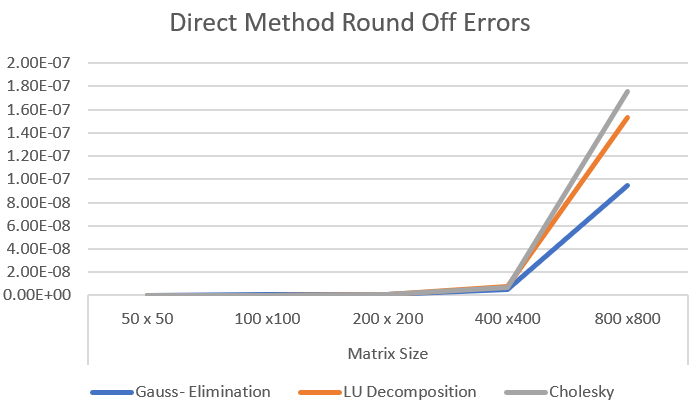
\includegraphics[width=\linewidth]{direct method round off errors}
    \caption{Arithmetic Floating Point Error }
    \label{fig:my_label}
\end{figure}
While we would expect direct methods(discussed below) such as Gauss, LU and Cholesky to generate an exact solution, we can see through our analyses that, due to nature of computer based computations that cause issues when floating point arithmetics are under consideration, the absolute errors in these methods, that we would theoretically expect to be zero, are not observed to be so. The errors tend to grow with increase in matrix size as more computations are required. 
\subsection{Dense Vs Sparse Solvers}
While the sparsity of matrices does not affect the performance of the solvers, when a sparse matrix is stored and iterated upon using the compressed sparse row format implemented in the CSR class, we can see the efficiency (both in terms of speed but especially memory used) improve drastically. This was especially notable when we analysed and compared the a diagonally dominant sparse matrix solved using the Jacobi dense versus the Jacobi Sparse method as shown in the table below.
\begin{table}[H]
\caption{Solving a Sparse Diagonally Dominant Matrix with a Dense Vs Sparse Jacobi Solver}
\label{tab:my-table}
\resizebox{\columnwidth}{!}{%

\begin{tabular}{@{}lllll@{}}
\toprule
\rowcolor[HTML]{DAE8FC} 
 & \multicolumn{2}{l}{\cellcolor[HTML]{DAE8FC}Jacobi Dense} & \multicolumn{2}{l}{\cellcolor[HTML]{DAE8FC}Jacobi Sparse} \\ \midrule
\rowcolor[HTML]{DAE8FC} 
Matrix Size                            & 100x100           & 200x200           & 100x100          & 200x200          \\
\cellcolor[HTML]{ECF4FF}Time           & 0.004             & 0.02              & 0.002            & 0.007            \\
\cellcolor[HTML]{ECF4FF}Absolute Error & 3.20747x$10^{-9}$ & 1.67387x$10^{-8}$ & 5.9555x$10^{-7}$ & 6.54x$10^{-7}$   \\
\cellcolor[HTML]{ECF4FF}Relative Error & 1.5059x$10^{-9}$  & 2.9288x$10^{-9}$  & 1.3305x$10^{-7}$ & 9.0728x$10^{-8}$ \\
\cellcolor[HTML]{ECF4FF}Iterations     & 12                & 15                & 15               & 13               \\ \bottomrule
\end{tabular}
}
\end{table}
From the table above, we observe that the Jacobi Sparse solver is indeed faster for both matrix sizes tested, however it can be noted that it is considerably faster for the 200x200 matrix. This aligns with our theoretical predication that for a sparse matrix as the matrix size increases, a sparse solve will be much more efficient in time and memory. One additional point to be noted is the fact that for a sparse matrix, we would need to compute the symbolic matmatmult to find the number of non-zero elements. This is an additional function that needs to be accounted for in sparse calculations. 
\subsection{Time and Matrix Size Analysis}

\begin{figure}[H]
    \centering
    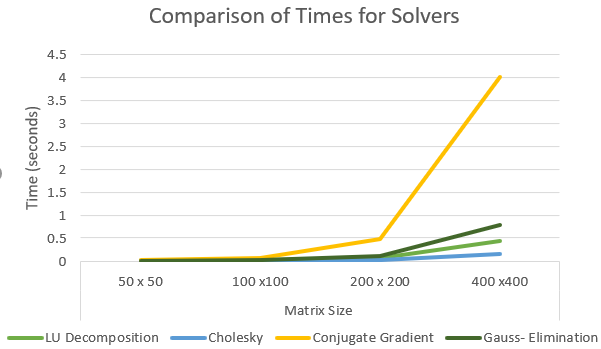
\includegraphics[width=\linewidth]{Times for Solvers}
    \caption{Times for Solvers}
    \label{fig:my_label}
\end{figure}

From the graph above we can see that from amongst the direct solvers, Gauss elimination takes greater  time to generate out compared to Cholesky and LU decomposition while conjugate gradient, an iterative solver, converges the slowest. Since iterative methods such as conjugate gradient tend to be faster for larger matrix sizes, we can speculate based on the data generated that a) the matrices we generated were not large enough to see the payoffs of an iterative method. b) Our compiler in Visual Studio optimized very well the direct methods but found the iterative method more challenging to optimize during runtime or c) conjugate gradient was sensitive to the generated inputs. 

\subsection{Memory and CPU Considerations}
\begin{figure}[H]
    \centering
    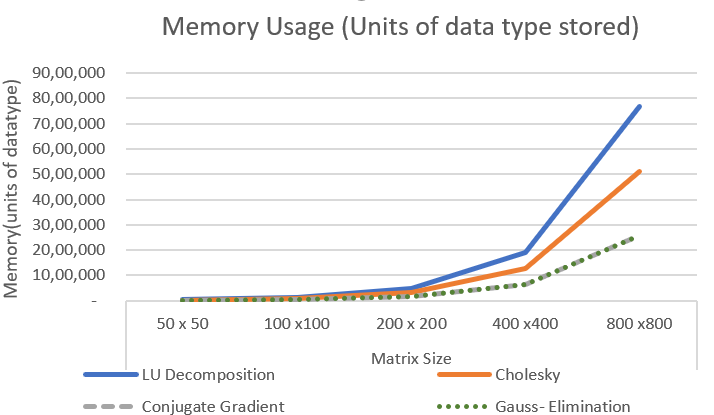
\includegraphics[width=\linewidth]{Memory usage for solvers}
    \caption{Caption}
    \label{fig:my_label}
\end{figure}
\begin{table}[H]
\caption{Average Memory(in units of memory) needed to Implement Solvers}
\label{tab:my-table}
\resizebox{\columnwidth}{!}{%
\begin{tabular}{llllll}
\hline
\rowcolor[HTML]{DAE8FC} 
Matrix Size                                & 50 x 50 & 100 x100 & 200 x 200 & 400 x400 & \cellcolor[HTML]{DAE8FC}800 x800 \\ \hline
\cellcolor[HTML]{ECF4FF}Gauss- Elimination & 2,600   & 10,200   & 40,400    & 1,60,800 & 6,41,600                         \\
\cellcolor[HTML]{ECF4FF}LU Decomposition   & 7,700   & 30,400   & 1,20,800  & 4,81,600 & 19,23,200                        \\
\cellcolor[HTML]{ECF4FF}Cholesky           & 5,150   & 20,300   & 80,600    & 3,21,200 & 12,82,400                        \\
\cellcolor[HTML]{ECF4FF}Conjugate Gradient & 2,800   & 10,600   & 41,200    & 1,62,400 & 6,44,800                         \\ \hline
\end{tabular}
}
\end{table}

One of major issues upon which we see a clear contrast in our analyses is the theoretical memory usage of direct and iterative methods. 
In the analyses above, we observe that for the same randomly generated linear system, direct and iterative methods behave differently - especially across a range of matrix sizes.For the matrix sizes analysed, we observe that direct methods are considerably faster. Since unlike iterative methods they arrive at an exact solution, we do not use our computational power to reach convergence.Further, in direct methods, once the decomposition is complete in the first iteration, for subsequent iterations we need only to compute backward and/or forward substitutions to reach the solution. However because they decompose the matrix, we are required to store two(Cholesky) or three (LU Decomposition) matrices. Therefore as the size of input matrices increase, the required memory for storing the data grows at O($n^{2}$) or O($n^{3}$) as compared to O(n) for iterative methods. This eats up memory rapidly.
\subsection{Ill-Conditioned Matrices}
In the usage of all our systems, we assume our matrices to be non-singular as a precondition to using our linear solvers. However for systems that are almost, but not quite singular in nature, i.e ill conditioned systems, linear solvers can show unexpected behaviour. 
We considered three ill conditioned system - the Hilbert Matrix with a condition number(calculated in python using the scipy library) of 15613, the Rutishauser System with a condition number of 44490 and the Wilkinson System with a condition number of 2.16x$10^{16}$. \\ We can see from the calculation of this condition number that any small change in the inputs (i.e. the linear system ) we are intending to solve will result in drastically different outputs. The tables below show the analyses for the different systems tested  - both in python (for comparison purposes) and using our dense solvers.

\begin{table}[H]
\caption{Ill Condition Matrices}
\label{tab:my-table}
\resizebox{\columnwidth}{!}{%
\begin{tabular}{@{}lll@{}}
\toprule
\rowcolor[HTML]{DAE8FC} 
Output Matrix                  & Hilbert (4x4) matrix & Rutishauser           \\ \midrule
\rowcolor[HTML]{DAE8FC} 
Condition Number (Scipy)       & 15613.79             & 100 x100              \\ \midrule
\cellcolor[HTML]{ECF4FF} Direct Methods & [-4, 60, -180, 140]             & [223, 355, -646, 542] \\
\cellcolor[HTML]{ECF4FF}Gauss Siedel                                    & [-3.99, 59.99, -179.99, 139.99] & [223, 355, -646, 542] \\ \midrule
\cellcolor[HTML]{ECF4FF}Python & [-4 ,60, -180, 140]  & [223, 355, -646, 542] \\ \bottomrule
\end{tabular}
}
\vspace{-5mm}
\end{table}

The table above shows the results output by our solvers against the output obtained in python for Hilbert and Rutishauser. We see that for these systems our solvers are quite reliable. Thus we can see that even though the system maybe ill-conditioned to a certain extent, our solvers give us a reliable output. \\
However when the condition number is very large(as calculated in scipy), such as for Wilkinson's Matrix,we fail to get a reliable output. This is driven by the fact that the diagonal number in the last row of matrix is the smallest (non zero) value in matrix and tends to zero as we divide it further during factorisation. This is the reason that direct methods do not give a valid outputs and when the Cholesky Solver was used, we get invalid results. Thus we can conclude that for higher levels of ill-conditioning precautions (such as pre-conditioning the matrix inputs) must be taken to avoid these failures.

\begin{table}[H]
\caption{Wilkinson’s Matrix where our Solvers Fail}
\label{tab:my-table}
\resizebox{\columnwidth}{!}{%

\begin{tabular}{lll}
\cline{1-1}
\rowcolor[HTML]{DAE8FC} 
Output Matrix & \begin{tabular}[c]{@{}l@{}}Wilkinson\\ (before perturbation)\end{tabular} & \begin{tabular}[c]{@{}l@{}}Wilkinson\\ (after perturbations)\end{tabular} \\ \cline{1-1}
\rowcolor[HTML]{DAE8FC} 
Condition Number (Scipy)               & 2.16x$10^{16}$                        & 2.16x$10^{16}$                 \\
\cellcolor[HTML]{ECF4FF}Direct Methods and Gauss Siedel    & [1.10937, 59.2326, -500900, 5.04E+09] & [1, 1, 1, 1]                   \\
\cellcolor[HTML]{ECF4FF}Python results & [1.10937, 59.2326, -500900, 5.04E+09] & [1, 1, 1.00000001, 9.9994E-01]
\end{tabular}
}
\vspace{-5mm}
\end{table}
\section{ Comparative Analysis and Results}
Thus in terms of solver choice, the following three considerations are to be taken into account by the user :
a) Robustness/ the ability to solve for changing properties of a linear system;
b) Performance/ time taken by the solver to converge/produce an output and finally;
c) Computational cost in terms of memory management and consumption by the solver
Keeping under consideration these three parameters the following table enumerates our recommendations for solver selection based on the user's priority area of optimization.

\begin{table}[H]
\caption{Solver Selection Table}
\label{tab:my-table}
\resizebox{\columnwidth}{!}{%
\begin{tabular}{
>{\columncolor[HTML]{ECF4FF}}l l}
\hline
\cellcolor[HTML]{DAE8FC}Solver & \cellcolor[HTML]{DAE8FC}Solver Order (Best to Worst)                                                                                                   \\ \hline
Robustness                     & \begin{tabular}[c]{@{}l@{}}\\Cholesky > LU Decomposition > Gauss Elimination > \\ Conjugate Gradient > Gauss-Siedel > Jacobi\end{tabular} \\ \\
Speed                          & \begin{tabular}[c]{@{}l@{}}Conjugate Gradient > Gauss-Siedel > Jacobi > \\ Cholesky > LU Decomposition > Gauss Elimination\end{tabular} \\ \\
\cellcolor[HTML]{ECF4FF}Memory Usage &
  \begin{tabular}[c]{@{}l@{}}Gauss -Siedel > Jacobi > Conjugate Gradient > \\ Cholesky, LU Decomposition, Gauss Elimination)\end{tabular}
\end{tabular}
}
\vspace{-4mm}
\end{table}

%------------------------------------------------

\section{Discussion on Further Improvements in Code}
\begin{itemize}
\item In terms of code structure, we could further improve our code by splitting the testing file into tests for developer and tests for users. This will allow the Test class to be used as a development and validation tool for the next versions while still allowing the users of the library to perform validation and error testing. The test class can be further improved by encapsulating our code for validations and performance into callable functions. This will avoid code repetitions which is in line with good design principles. 
\item We can extend our functionalities to support other different types of input including banded matrices and other types of sparse solvers. This library could also be extended with more functionalities for matrix and CSR matrix operations such as finding getting and setting values, finding the diagonals etc.

\item There are certain errors in Read-Files function when handling matrices of very large sizes (such as 1000x1000). Better methods to generate and store inputs can be considered for more accurate and efficient computations.
\item For iterative solvers, other than the two stopping conditions we have considered (a tolerance  and a maximum number of iterations input by the user), to better understand the nature and usability of the results, there might be a strong reason to add a function that allows us to check for divergence. 
\end{itemize}


%----------------------------------------------------------------------------------------
%	REFERENCE LIST
%----------------------------------------------------------------------------------------
\begin{thebibliography}{99} 
\bibitem[1]{}Lecture 5 : MSc ACSE - Advanced Programming Coursework.
\newblock {\em Gauss Elimination and LU Decomposition}, .
 
 \bibitem[2]{} The Jacobi and Gauss-Seidel Iterative Methods and Imperial College London Library.
\newblock {\em Science Direct}.
\bibitem[3]{}An Introduction to the Conjugate Gradient Method Without the Agonizing Pain by Jonathan Richard Shewchuk.
\newblock {\em Edition 114}.

\bibitem[5]{}Notes on Cholesky Factorization Robert A. van de Geijn Department of Computer Science The University of Texas Austin

\bibitem[6]{}How to Generate Random Matrices from the Classical Compact Groups by Francesco Mezzadri.
\newblock {\em Volume 54, Number 5}.
\bibitem[7]{}What is Wilson Matrix, Nick Higham.
\newblock {\em https://nhigham.com/2021/06/01/what-is-the-wilson-matrix/}.

\end{thebibliography}
Yuna - Testing, Analysis, Gauss Siedel \quad \quad \quad \quad \quad \quad \quad \quad
Ellya - Cholesky, Conjugate Gradient, LU Decomposition,Jacobi, Analysis \quad \quad \quad
Niranjana - Gauss, Conjugate Gradient, Jacobi, Interface, Report
%----------------------------------------------------------------------------------------

\end{document}
